\subsection{The geometric significance of the dot product}

The \textbf{included angle}\index{included angle} of two vectors
$\vect{u}$ and $\vect{v}$ is the angle $\theta$ between the vectors
such that $0 \leq \theta \leq \pi$.
\begin{center}
  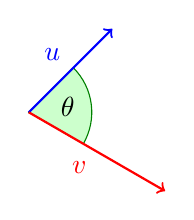
\begin{tikzpicture}
    \filldraw[fill=green!20,draw=green!50!black] (0,0) -- (-30:8mm) arc (-30:45:8mm) -- cycle;
    \draw[->, thick, blue](0,0) -- node[above left] {$\vect{u}$} (45:1.5);
    \draw[->, thick, red](0,0) -- node[below left] {$\vect{v}$} (-30:2);
    \node at (7.5:5mm){$\theta$};
  \end{tikzpicture}
\end{center}
The dot product can be used to determine the included angle between
two vectors.

\begin{proposition}{The dot product and the included angle}{dotproduct-angle}
  Let $\vect{u}$ and $\vect{v}$ be two vectors in $\R^n$, and let 
  $\theta$ be the included angle. Then the following equation holds.
  \begin{equation*}
    \vect{u}\dotprod \vect{v}=\norm{\vect{u}} \norm{\vect{v}} \cos \theta.
  \end{equation*}
\end{proposition}

In words, the dot product of two vectors equals the product of the
magnitude (or length) of the two vectors multiplied by the cosine of
the included angle. Note that this gives a geometric description of
the dot product that does not depend explicitly on the coordinates of
the vectors.

\begin{example}{Find the angle between two vectors}{angle-two-vectors}
Find the angle between the vectors
\begin{equation*}
  \vect{u}
  =
  \begin{mymatrix}{r}
    2 \\
    2
  \end{mymatrix}
  \quad\mbox{and}\quad
  \vect{v}
  =
  \begin{mymatrix}{r}
    0 \\
    3 
  \end{mymatrix}.
\end{equation*}
\end{example}

\begin{solution}
  By Proposition~\ref{prop:dotproduct-angle},
  \begin{equation*}
    \vect{u}\dotprod \vect{v}=\norm{\vect{u}} \norm{\vect{v}} \cos \theta.
  \end{equation*}
  Hence, 
  \begin{equation*}
    \cos \theta =\frac{\vect{u}\dotprod \vect{v}}{\norm{\vect{u}}\norm{\vect{v}}}.
  \end{equation*}
  First, we compute $\vect{u}\dotprod \vect{v} = (2)(0) + (2)(3) = 6$.
  Then, 
  \begin{equation*}
    \begin{array}{l}
      \norm{\vect{u}} = \sqrt{2^2+2^2}=\sqrt{8},\\
      \norm{\vect{v}} = \sqrt{0^2+3^2}=3.
    \end{array}
  \end{equation*}
  Therefore, we have
  \begin{equation*}
    \cos \theta =\frac{6}{3\sqrt{8}} = \frac{1}{\sqrt{2}}.
  \end{equation*}
  Taking the inverse cosine of both sides of the equation, we find
  that $\theta =\frac{\pi}{4}$ radians, or 45 degrees.
\end{solution}

\begin{example}{Computing a dot product from an angle}{geometric-dot-product}
  Let $\vect{u},\vect{v}$ be vectors with $ \norm{\vect{u}} = 3$ and $\norm{\vect{v}} = 4$. 
  Suppose the angle between $\vect{u}$ and $\vect{v}$ is $\pi / 3$. Find $\vect{u}\dotprod \vect{v}$.
\end{example}

\begin{solution}
  From Proposition~\ref{prop:dotproduct-angle}, we have
  \begin{equation*}
    \vect{u}\dotprod \vect{v}
    =\norm{\vect{u}} \norm{\vect{v}} \cos \theta
    =3\cdot 4\cdot \cos\tup{\frac{\pi}{3}}
    =3\cdot 4\cdot \frac{1}{2}=6.
\end{equation*}
\end{solution}

% ----------------------------------------------------------------------
\subsection{Orthogonal vectors in $\R^n$}

Two nonzero vectors are said to be
\textbf{orthogonal}\index{vector!orthogonal}\index{orthogonal vectors},
sometimes also called
\textbf{perpendicular}\index{vector!perpendicular}\index{perpendicular vectors},
if the included angle is $\pi /2$ radians ($90^{\circ })$. By
convention, we also say that the zero vector is orthogonal to all
vectors.

\begin{proposition}{Orthogonal vectors}{perp-vectors}
  Let $\vect{u}$ and $\vect{v}$ be vectors in $\R^n$. Then $\vect{u}$
  and $\vect{v}$ are orthogonal\index{vector!orthogonal} if and only
  if
  \begin{equation*}
    \vect{u} \dotprod \vect{v} = 0.
  \end{equation*}
\end{proposition}

\begin{proof}
  If $\vect{u}$ or $\vect{v}$ is zero, the vectors are orthogonal by
  definition, and the dot product is $0$ in that case, so the
  proposition holds. Now assume $\vect{u}$ and $\vect{v}$ are both
  non-zero.  Then by Proposition~\ref{prop:dotproduct-angle}, we have
  $\vect{u} \dotprod \vect{v} = 0$ if and only if
  $\norm{\vect{u}} \norm{\vect{v}} \cos \theta$ if and only if
  $\cos\theta=0$. Recall that the included angle is between $0$ and
  $\pi$. Therefore, $\cos\theta=0$ if and only if $\theta=\pi/2$.
\end{proof}

\begin{example}{Determine whether two vectors are orthogonal}{orthogonal-vectors}
Determine whether the vectors
\begin{equation*}
\vect{u}=
\begin{mymatrix}{r}
2 \\
1 \\
-1 
\end{mymatrix}
\quad\mbox{and}\quad
\vect{v} 
=
\begin{mymatrix}{r}
1 \\
3 \\
5
\end{mymatrix}
\end{equation*}
are orthogonal.
\end{example}

\begin{solution}
  In order to determine if these two vectors are orthogonal, we
  compute the dot product. We have
  \begin{equation*}
    \vect{u} \dotprod \vect{v}
    =
    (2)(1) + (1)(3) + (-1)(5)
    =
    0,
  \end{equation*}
  and therefore, by Proposition \ref{prop:perp-vectors}, the two vectors are orthogonal.
\end{solution}
